\documentclass[12pt,border=3mm]{standalone}% <<<---
\usepackage{tikz}
\usetikzlibrary{positioning,shapes.misc}

%\tikzset{% <<<--- became irrelevant from REFACTORING
%  figNode/.style={
%    path picture={
%      \node at (path picture bounding box.center) {#1};}}
%}

% ~~~ macros (shorthand notations) from REFACTORING ~~~~~~~~~~~~~~~~~~~~~~~
\newcommand\graybox[1]{\draw[cmnbox] #1 rectangle ++(7,3.5);}% the gray boxes

\newcommand\colcirc[3]{% #1=color, #2=nodes name, #3=text
    \draw[#1]      (#2) circle (1);%
    \node [font=\Large]     at (#2) {#3};}% to put text, like 2, ch 2 etc.

% ~~~~~~~~~~~~~~~~~~~~~~~~~~~~~~~~~~~~~~~~~~~~~~~~~~~~~~~~~~~~~
\begin{document}

  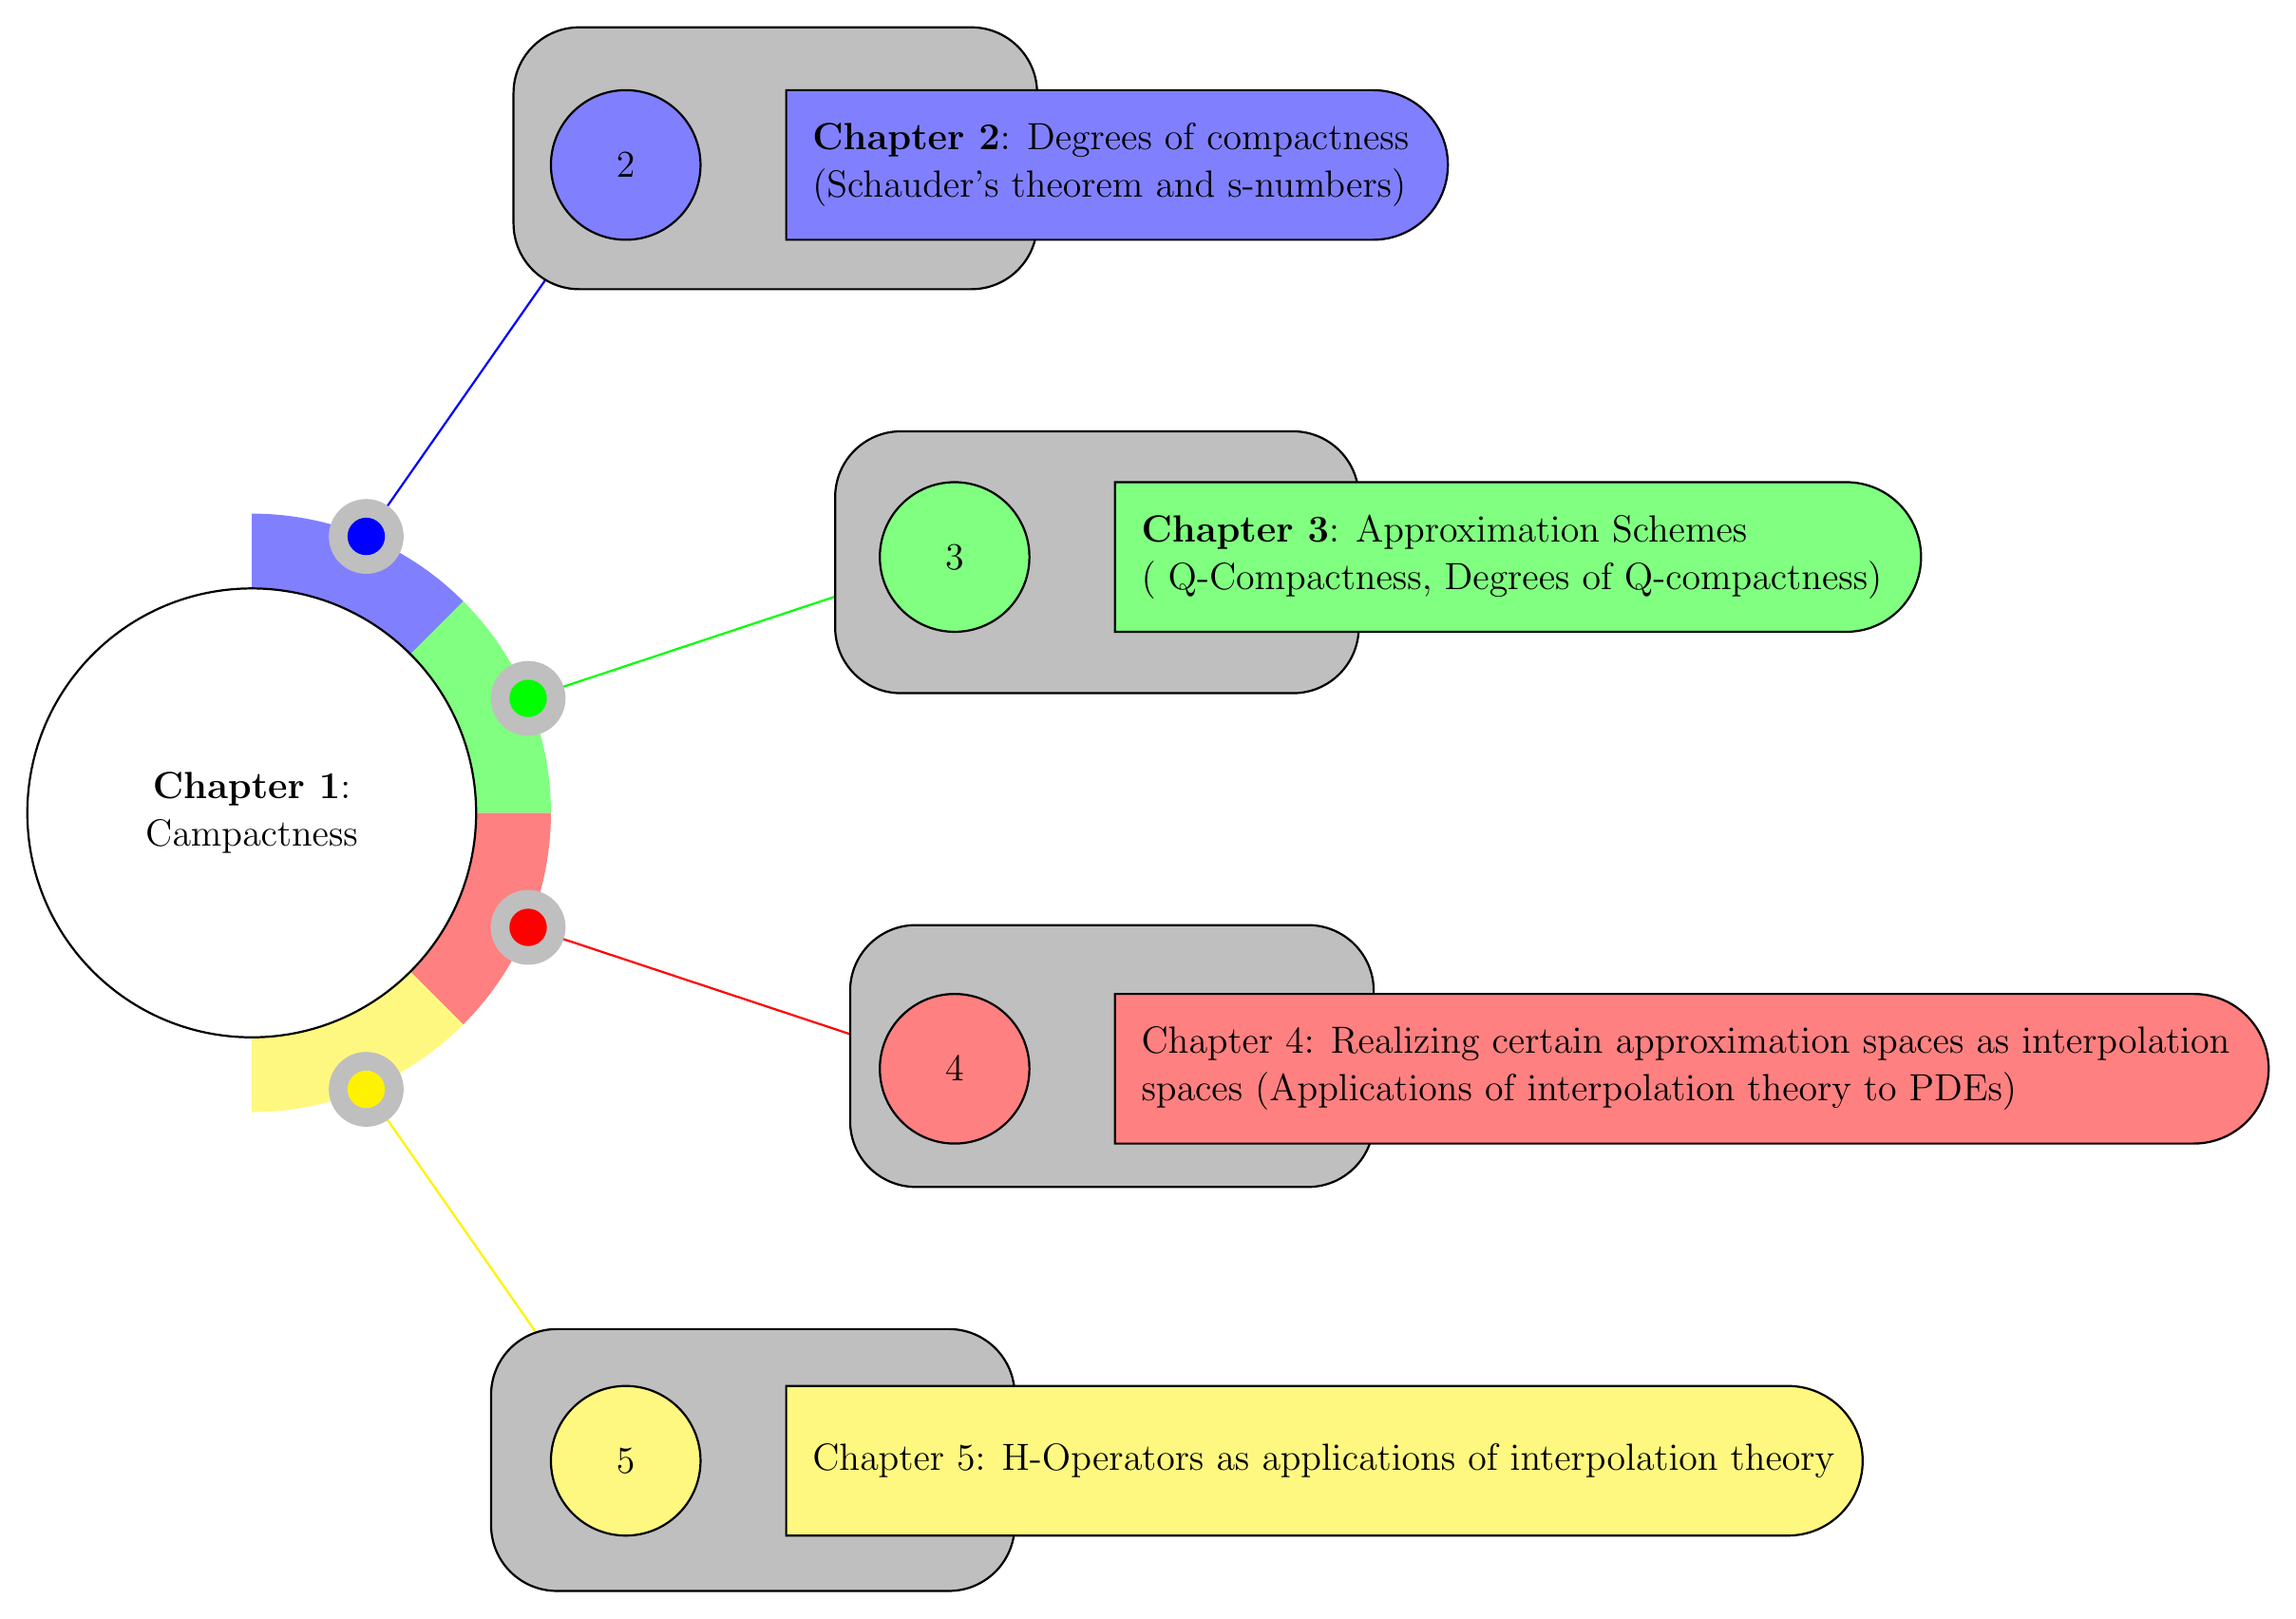
\begin{tikzpicture}
    [thick,
    cmnnode/.style={rounded rectangle=25pt,% common node style
                    rounded rectangle west arc=none,
                    draw,
                    minimum height=2cm, minimum width=3cm,% these you had already
                    font=\Large,% larger fonts; \LARGE would be maximum
                    align=left,% for multilines, indicated by \\
                    inner sep=1em% give it a bit more space to breath
                    },
    cmnbox/.style= {rounded corners=25pt,% common box style
                    fill=gray!50}
    ]
    \node (a) at (60:10){};
    \node (b) at (20:10){};
    \node (c) at (-20:10){};
    \node (d) at (-60:10){};
    %\node (e) at (-80: 10){};
  
    % ~~~ colored arc segments ~~~~~~~~~~~~~~~~~~~~
    \foreach \r/\c in {90/blue,45/green,0/red,-45/yellow}{
      \fill[\c!50] (0,0) -- (\r:4) arc (\r:\r-45:4) -- cycle;
    };
  
    % ~~~ small gray and colored circles ~~~~~~~~~~~~~~
    \foreach \r/\c/\p in {67.5/blue/a,22.5/green/b,-22.5/red/c,-67.5/yellow/d}{
      \draw[\c]         (\r:4) -- (\p);
      \fill[gray!50]    (\r:4) circle (0.5);
      \fill[\c]         (\r:4) circle (0.25);
    };
  
    % ~~~ root-circle ~~~~~~~~~~~~~~~~
    \draw[fill=white,font=\Large] (0,0) circle (3) node[align=center]{\textbf{Chapter 1}:\\ Campactness};% augmented: font, \\ (multiline), \textbf{} for bold text-part 
  
    % ~~~ 1st, blue ~~~~~~~~~~~~~~~~
    \graybox{(3.5,7)}               % simplified, see macro above
    \colcirc{fill=blue!50}{a}{2}    % simplified, see macro above
    % reusing common node style, some bold text, \\ (multiline)
    \node[right=2 of a, cmnnode, fill=blue!50] {\textbf{Chapter 2}: Degrees of compactness\\(Schauder's theorem and s-numbers)};
  
    % ~~~ 2nd, green ~~~~~~~~~~~~~~~~~
    \graybox{(7.8,1.6)}
    \colcirc{fill=green!50}{b}{3}
    \node[right=2 of b, cmnnode, fill=green!50] {\textbf{Chapter 3}: Approximation Schemes\\( Q-Compactness, Degrees of Q-compactness) };
  
    % ~~~ 3rd, red ~~~~~~~~~~~~~~~~~
    \graybox{(8,-5)}
    \colcirc{fill=red!50}{c}{4}
    \node[right=2 of c, cmnnode, fill=red!50] {Chapter 4: Realizing certain approximation spaces as interpolation\\spaces (Applications of interpolation theory to PDEs)};
  
     % ~~~ 4th, yellow ~~~~~~~~~~~~~~~~~~~~~
    \graybox{(3.2,-10.4)}
    \colcirc{fill=yellow!50}{d}{5}
     \node[right=2 of d, cmnnode, fill=yellow!50] {Chapter 5: H-Operators as applications of interpolation theory};
    
    
  \end{tikzpicture}
\end{document}